
% this file is called up by thesis.tex



\chapter{Material \& Metoder} % top level followed by section, subsection
\label{ch:metoder}

% ----------------------- paths to graphics ------------------------

% change according to folder and file names
\ifpdf
    \graphicspath{{8/figures/PNG/}{8_materials_and_methods/figures/PDF/}{8_materials_and_methods/figures/}}
\else
    \graphicspath{{8/figures/EPS/}{8_materials_and_methods/figures/}}
\fi

% ----------------------- contents from here ------------------------



\section{Metoder}
För att öka tryggheten för väntande bussresenärer utvecklades ett system för att detektera närvaro.\\

En vibrationssensor användes först men den var för känslig så vibrationssensorn ersattes med en PIR-sensor istället. När värdet från PIR-sensorn överskred ett tröskelvärde så tändes en lampa. Lampan var tänd en viss förutbestämd tid innan den släcktes. Denna systemlösningen kommer att användas när aktiv övervakning ska ske.\\

För att upptäcka vandalisering av busshållplatsen användes en ljud-sensor. \\

IP-kameran var installerad i mitten av vägen för att först filma hållplatsen och sen omgivningen runt hållplatsen. Detta är viktigt eftersom vandaliseringen kan ske på avstånd.\\

En schemaläggare användes för att hela systemet skulle fungera samtidigt så att komponenter inte begränsade varandra. Varje komponent turades om en begränsad tid att vara aktiv. Detta var nödvändigt att göra eftersom sensorer skulle lyssna kontinuerligt på förändringar hos omgivningen medan systemet var aktivt och utförde andra uppgifter.\\

En FTP-server upprättades för att kunna ta emot videoinspelningar från IP-kameran . När IP-kameran aktiverades så filmade kameran 5 sekunder och sen ett helt varv på ytterligare 30 sekunder. \\

Det finns totalt tre tasks i systemet som exekveras parallellt för att kunna låta processorn jobba med flera saker samtidigt. Biblioteket som möjliggör att dessa tasks arbetar oberoende av varandra och som detta systemet använde sig av skapades av Nicholas Wiersma och heter ESP8266Scheduler. Två av de tre tasksen(pirsensorn och ljudsensorn) agerar som inputs till systemet. Den tredje tasken (WifiTask) kontrollerar om det finns en wifi-anslutning, om anslutningen är nere försöker den återansluta.

\begin{figure}[h]

  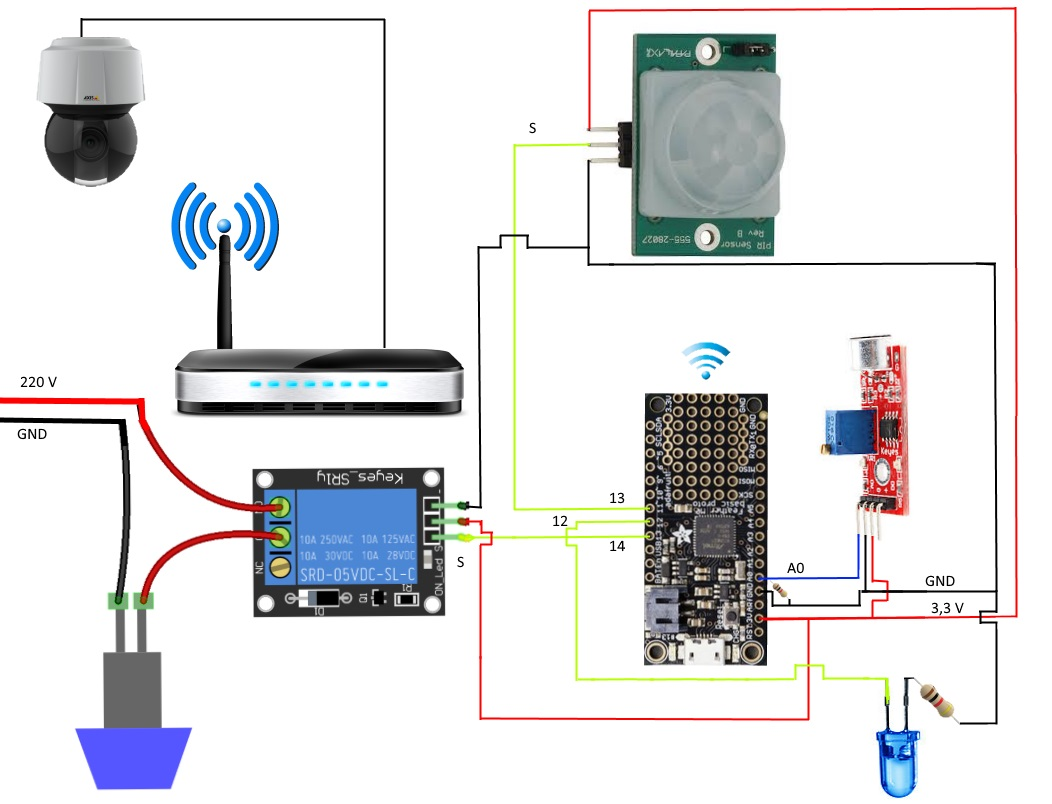
\includegraphics[width=\linewidth]{connections.jpg}
  \caption{Alla komponenter kopplade med varandra.)}
  \label{fig:connections}
\end{figure}



\section{ESP8266 - mikroprocessorn}
Huvudanledningen för valet av denna mikroprocessor var att den hade en inbyggd Wifi-mottagare vilket var absolut nödvändigt för att kunna kommunicera med nätverket där kameran var uppkopplad. Givetvis kunde gruppen hitta på alternativa lösningar men just denna lösning var den smidigaste. Det fanns tillräckligt med både digitala ingångar och en analog ingång. Den analoga ingången klarar en spänning på 1V.\\

Sensorer kopplades till ESP:n och ESP:n kommunicerade med kameran via wifi-anslutning.\\

Svårigheten som uppstod var hanteringen av avlästa sensor värden med avseende på tid och periodicitet. Koden nedan visar hur gruppen fick sina värden:

\begin{lstlisting}
const int pirSen = 13; // Digital pin for pir sensor
...
pinMode(pirSen, INPUT); // The pin is set as INPUT
...
int pirValue = digitalRead(pirSen); // Gets a reading from the pin
\end{lstlisting}
Efter flera tester och noteringar kom gruppen fram till ett counter-system för att hantera sensorns digitila värden.
\begin{lstlisting}
void doWithPirValue(int pirvalue) {
  if (pirvalue == HIGH){
    pirCounter = pirCounter + 1; // Counter for each reading
    pirSum = pirSum + 10; // Sum-counter for each HIGH value reading
  }

  if (pirvalue == LOW){
    pirCounter = pirCounter + 1; // Counter for each reading
  }
}

void doWhenMove() {
  if (pirCounter == 7) {
    pirCounter = 0; // Reset for the counter of each reading
    if (pirSum == 70) {
      prevTime = millis(); // Timer to put light on
      digitalWrite(pirLed, HIGH); // Big light ON
    }
    if (pirSum < 70 && ( millis()  - prevTime ) > 10000 ) {
      digitalWrite(pirLed, LOW); // Big light OFF
      prevTime = 0; // Reset for the timer 
    }
    pirSum = 0; // Reset for the sum-counter of HIGH value readings
  }  
}
\end{lstlisting}
ESP:n läste av ljud-sensorn (mikrofonen) analogt. Det uppstod under demo-dagen ett problem där mikrofonen hela tiden gav höga analoga värden. Det berodde på att sensorn hängde upp och ner och vid montering under redovisningen hade sladden från mikrofonen till ESP:n lossnat vilket medförde att ESP:n läste in analoga värden på 1023. Det löstes genom att filtrera bort analoga värdet på 1023 i koden med en if-sats och kopplade ESP:ns analoga pin till jord via en resistor. Resistorn hade en hög resistans så den inte påverkade sensorns avläsning. Koden nedan visar hur sensorn läser in sina värden.

\begin{lstlisting}
const int micSen = A0; // Analogpin for the pir sensor 
const int micLed = 12; // Small lamp for mic-action

int sensorValue = analogRead(micSen); // Gets an analog reading

void doWithSensorValue(int sensorvalue) {
  
  if ( sensorvalue < 1023 ) { // To make sure of correct reading
    if (sensorvalue > 71) { // limit value to alert
        digitalWrite(micLed, HIGH); // MIC light ON
    }
    if (sensorvalue < 72) { // limit value to non-alert
        digitalWrite(micLed, LOW); // MIC light OFF
    }
  }
  
}
\end{lstlisting}

\section{FTP-Server}
För att kunna identifiera personer begår vandalisering måste systemet lagra bilder/inspelningar på en server. En FTP-server användes. FTP-servern och IP-kameran låg under samma subnät.\\

Information om FTP-servern:

\begin{itemize}
\item IP adress : 192.168.0.106

\item Port nummer : 21

\item Användarnamn : ”FTP-User”

\item Lösenord : ”Safe24”

\end{itemize}
\section{IP-kameran}
Kameran är av modellen Q6128-E Network Camera med möjlighet till internetuppkoppling. Upplösningen som används är 3840x2860. Ett suffix med datum och tidsinformation läggs till i filnamnet för inspelningen.\\

IP-kameran användes för att skicka bilder och video till en server för datalagring.\\

Kommunikationen med kameran gjordes via ESP8266 som sände kommandon över internet för att styra kameran.\\

Tre events skapades; "ActionPTZStation1", "ActionRecord", "ActionPTZHome".\\

ActionPTZStation1: När virtuell port X aktiveras så riktas kameran till en bestämd position som heter "plats1" (busshållplatsen).\\

ActionRecord: När virtuell port 9 aktiveras så börjar kameran videoinspelningen. Efter avslutad inspelning skickas inspelningen till FTP-servern. \\

ActionPTZHome: När virtuell port X aktiveras så riktas kameran till en bestämd position som heter "Safe24" och motsvarar start och slutpositionen för kameran.\\

\section{Sensorer}
En PIR-sensor från Adafruit användes som rörelsedetektor för att lysa upp den stora lampan. Den kopplades till ESP:n via tre sladdar, en röd som gick till strömmen, trots att det krävdes minst 5 V så gick det bra med 3,3 V från ESP:n. Den andra sladden gick till jord och den tredje är själva signalsladden som då gick till en digital pin som var satt till input-mode. För att gruppen skulle lyckas med pir-sensorn fick de med hjälp av delay och en counter räkna in hur många gånger som signalen är hög eller låg. Efter flera tester och försök kom de fram till att det behövdes minst 7 rundor där en runda är på 0,5 s. Anledningen till detta var att näär det inte fanns rörelse så gav PIR-sensor utsalg med 6 ettor och en nolla. Då det fanns rörelse gav den utslag på bara ettor. Slutligen gällde det att om programmmet läste in 7 värden från signal-pin, så skulle summan vara 7 vid rörelse och om summan var under sju betydde det att ett av värden var noll, alltså ingen rörelse. Ibland kom det även störningar som gjorde att PIR-sensorn bara visade ettor, vilket senare fram i tiden löstes genom att utföra en digitalWrite på PIR-input-pin:n med värdet låg.  \\

\begin{figure}[h]

  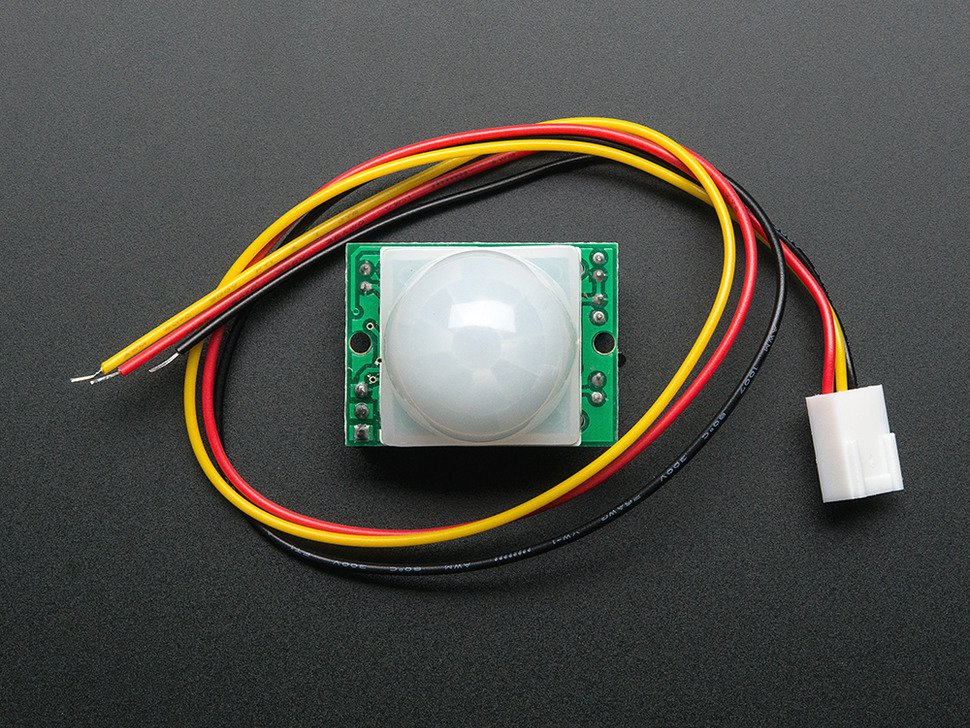
\includegraphics[width=\linewidth]{pir.jpg}
  \caption{En PIR-sensor från Adafruit. (www.adafruit.com)}
  \label{fig:pir}
\end{figure}
PIR-sensorn registrerade ifall det förekom någon rörelse. Denna sensorn skickade digitala värden till ESP8266.\\

På grund av vibrationssensorn var så känslig använde gruppen en ljudsensor istället som hade mikrofon. På samma sätt som PIR-sensor kopplades den till ström och jord och en tredje sladd gick till analog-pin istället för en digital. Eftersom en digital pin gav antingen en låg eller hög signal, dvs antingen en etta eller en nolla, medan den analoga pin:n gav olika heltals-väärden beroende på styrkan av signalen, som egentligen motsvarade för högre spänning. 
Glas har så som andra material en naturlig resonansfrekvens med vilken material oscillerar eller enklare sagt vibrerar. Självklart varierar denna frekvens från typ till annan beroende av glasets form och om det innehåller något dämpande. Ljud som har samma ton som den naturliga frekvensen kan få glas att börja vibrera. Det krävs även en hel del ”styrka” vid sidan av tonen. Ju högre ljudet är desto mer vibrerar glaset, och vid en viss gräns kommer inte glaset att tåla dessa vibrationer och därför går glaset i sönder. Det krävs att man kommer upp till över 100 dB. Det säger egentligen inte mycket, om man inte vet i förväg att en människas normala tal är runtomkring 50 dB. 

På grund av brist på glas och utrymme för gruppen för att de skulle  göra försök att ta i sönder glas hade de bestämt i detta projekt att utgå från slag mot en kartong eller en miniatyr av en hållplats med en gräns på 75 dB. Över denna gräns betydde det att de har glas som hade gått i sönder.\\
\begin{figure}[h]

  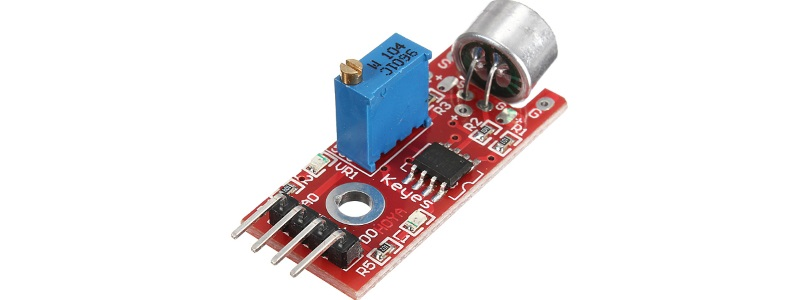
\includegraphics[width=\linewidth]{mic.jpg}
  \caption{En ljudsensor med mikrofon. (www.bazaargadgets.com)}
  \label{fig:mic}
\end{figure}
\clearpage
\section{Systembeskrivning}
Nu har gruppen beskrivit olika delar av systemet och hur dem används. Om PIR-sensor detekterar någon rörelse då skall lampan ska tändas en viss tid och sedan släckas, så länge sensorn inte detekterar en ny rörelse. Ljud-sensorn är också igång hela tiden. Om ljudsensor detekterar ett ljud som är över gränsvärdet ska den viktiga processen börja. Först aktiveras två virtuella porter i kameran. Den ena riktar kameran mot busshållplatsen och den andra gör att kameran börjar filma och filmen skickas till FTP-servern. Videolängden är 40 sekunder och efter 5 sekunder börjar kameran att filma runt omkring dvs kameran ska börja vrida sig horisontellt. Ett varv tar cirka 27 sekunder dvs efter 33 sekunder ska kameran riktas mot busshållplatsen igen och det görs genom att aktivera en virtuell port. Kameran ska forsätta filma cirka 7 sekunder till och efter det ska den riktas mot sitt standardläge dvs "homeposition". Ifall ljud sensor detekterar ett annat ljud som är över gränsen inom 40 sekunder då ska processen börja från början dvs kameran riktas tillbaka mot bushållplatsen, ska börja vrida efter 5 sekunder osv. Det enda som blir annorlunda vid detektering av två ljud inom 40 sekunder blir videolängden. Till exempel om ett annat ljud detekteras 15 sekunder efter första ljud då blir videolängden 40+15 sekunder dvs 55 sekunder.\\
Gruppen var väl medvetna om att ljudsensorn inte var det bästa valet för systemet, dock var den, den mest tillgängliga. Vid besök hos en elektrokit-grossist kunde de inte få tag på någon användbar trycksensor som var tillräckligt känslig för att ersätta ljudsensorn. Under demo-dagen fick de frågan om de hade tänkt på en Piezo-sensor, vilken är en typ av en tryck-sensor. Efter fakta-sökning fann gruppen att en Piezo-sensor hade varit ett bättre alternativ än ljudsensorn.

\section{Arbetsuppgifter}
Gruppen arbetade både tillsammans och även enskilt så att var och en av gruppmedlemmarna kunde bidra med något. Benjamin var delaktig i arbetet med flödesdiagram, tasks, hjälp med byggandet av busshållplats och även testfall. Yurdaer arbetade med wifi-kodning av ESP:n, kamera-kommandon, ftp-servern och i rapporten skrev han om sina delar samt om etiska aspekter. Georges bidrag var med struktur av kod, API, manual, testfall, FTP-servern och en del rapportskrivning. Han bidrog även med upprättande av en Latex-mall för rapporten. Louay arbetade med sensorernas kodning, ihopkoppling av alla komponenter, förslag till router-lösning, byggandet av en hållplats och kontinuerlig testning av alla kopplingar. 
% ---------------------------------------------------------------------------
%: ----------------------- end of thesis sub-document ------------------------
% ---------------------------------------------------------------------------



 



